%-------------------------
% Resume in Latex
% Author : Sourabh Bajaj
% License : MIT
%------------------------

\documentclass[a4paper,11pt]{article}

\usepackage{latexsym}
\usepackage[empty]{fullpage}
\usepackage{titlesec}
\usepackage{marvosym}
\usepackage[usenames,dvipsnames]{color}
\usepackage{verbatim}
\usepackage{enumitem}
\usepackage[hidelinks]{hyperref}
\usepackage{fancyhdr}
\usepackage[english]{babel}
\usepackage{tabularx}
\usepackage{graphicx}
\usepackage{color}
\usepackage{xcolor}
\usepackage{tgbonum}
\usepackage[margin=1.4in]{geometry}
\usepackage{setspace}
\input{glyphtounicode}

\pagestyle{fancy}
\fancyhf{} % clear all header and footer fields
\fancyfoot{}
\renewcommand{\headrulewidth}{0pt}
\renewcommand{\footrulewidth}{0pt}

\hypersetup{breaklinks=true,%
% pagecolor=white,%
colorlinks=true,%
linkcolor=MyBlue,%
urlcolor=MyBlue}


\definecolor{MyBlue}{rgb}{0.25, 0.41, 0.88}

% Adjust margins
\addtolength{\oddsidemargin}{-0.5in}
\addtolength{\evensidemargin}{-0.5in}
\addtolength{\textwidth}{1in}
\addtolength{\topmargin}{-.5in}
\addtolength{\textheight}{1.0in}

\urlstyle{same}

\raggedbottom
\raggedright
\setlength{\tabcolsep}{0in}

% Sections formatting
\titleformat{\section}{
  \vspace{-4pt}\scshape\raggedright\large
}{}{0em}{}[\color{black}\titlerule \vspace{-5pt}]

% Ensure that generate pdf is machine readable/ATS parsable
\pdfgentounicode=1

%-------------------------
% Custom commands
\newcommand{\resumeItem}[2]{
  \item\small{
    \textbf{#1: }{#2 \vspace{-2pt}}
  }
}

% Just in case someone needs a heading that does not need to be in a list
\newcommand{\resumeHeading}[4]{
    \begin{tabular*}{0.99\textwidth}[t]{l@{\extracolsep{\fill}}r}
      \textbf{#1} & #2 \\
      \textit{\small#3} & \textit{\footnotesize #4} \\
    \end{tabular*}\vspace{-5pt}
}

\newcommand{\resumeSubheading}[4]{
  \vspace{-1pt}\item
    \begin{tabular*}{0.97\textwidth}[t]{l@{\extracolsep{\fill}}r}
      \textbf{#1} & #2 \\
      \textit{\footnotesize #3} & \textit{\footnotesize #4} \\
    \end{tabular*}\vspace{-5pt}
}

\newcommand{\resumeSubSubheading}[2]{
    \begin{tabular*}{0.97\textwidth}{l@{\extracolsep{\fill}}r}
      \textit{\footnotesize #1} & \textit{\footnotesize #2} \\
    \end{tabular*}\vspace{-5pt}
}

\newcommand{\resumeSubItem}[2]{\resumeItem{#1}{#2}\vspace{-4pt}}

\renewcommand{\labelitemii}{$\circ$}

\newcommand{\resumeSubHeadingListStart}{\begin{itemize}[leftmargin=*]}
\newcommand{\resumeSubHeadingListEnd}{\end{itemize}}
\newcommand{\resumeItemListStart}{\begin{itemize}}
\newcommand{\resumeItemListEnd}{\end{itemize}\vspace{-5pt}}

% Own symbols
\newcommand{\CC}{C\nolinebreak\hspace{-.05em}\raisebox{.4ex}{\tiny\bf +}\nolinebreak\hspace{-.10em}\raisebox{.4ex}{\tiny\bf +}}
\def\CC{{C\nolinebreak[4]\hspace{-.05em}\raisebox{.4ex}{\tiny\bf ++}}}
\newcommand{\mytextsharp}{$^\sharp$}

%-------------------------------------------
%%%%%%  CV STARTS HERE  %%%%%%%%%%%%%%%%%%%%%%%%%%%%

\begin{document}

%----------HEADING-----------------
%\begin{figure}[htbp]
%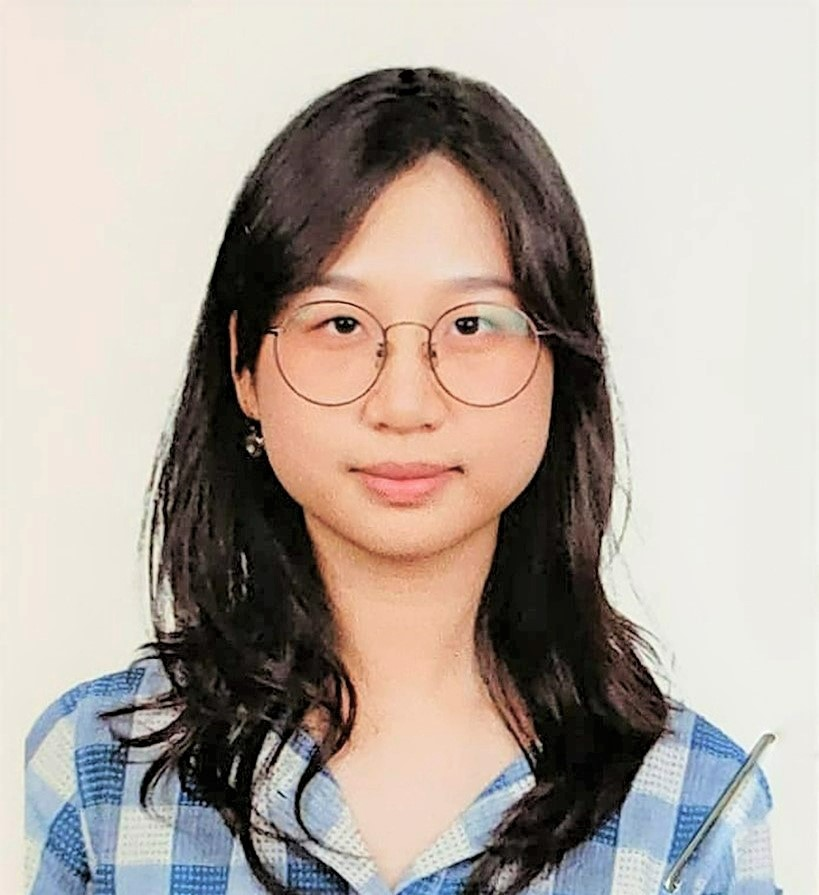
\includegraphics[width=1.5cm]{profile-pic.jpg}
%\begin{tabular*}{\textwidth}{l@{\extracolsep{\fill}}r}
%  \textbf{{\Large LIANA LING}} & Email : \href{mailto:lianalingliya@gmail.com}{lianalingliya@gmail.com}\\
%  \href{http://github.com/lianaling/}{GitHub Profile} & Mobile : +60 17-280 1215 \\
%\end{tabular*}
%\end{figure}

\begin{tabular*}{\textwidth}{l@{\extracolsep{\fill}}r}
  \textbf{{\LARGE LIANA LING}} & Email: \href{mailto:lianalingliya@gmail.com}{lianalingliya@gmail.com}\\
  \href{http://github.com/lianaling/}{A software engineering student's GitHub Profile} & Mobile: \href{tel:+60172801215}{+60 17-280 1215} \\
\end{tabular*}

%-----------EDUCATION-----------------
\section{Education}
\resumeSubHeadingListStart
\resumeSubheading
{Tunku Adbul Rahman University College}{Kuala Lumpur, Malaysia}
{Bachelor of Computer Science (Honours) in Software Engineering;}{Oct 2019 -- Oct 2022}
\begin{spacing}{0.4}
  \colorbox{yellow}{\it\footnotesize CGPA: 3.9744}
\end{spacing}
\resumeSubSubheading{Foundation in Science; CGPA: 4.0000}{Sep 2018 -- Sep 2019}
\resumeItemListStart
\resumeItem{Skills Learnt}{\CC, C\mytextsharp, Java, Python, ASP.NET, SQL, HTML/CSS/Javascript}
\resumeItem{Languages}{Proficient in written/spoken Chinese and English; Conversational in Malay}
\resumeItemListEnd
\resumeSubHeadingListEnd


%-----------EXPERIENCE-----------------

% --------Multiple Positions Heading------------
%    \resumeSubSubheading
%     {Software Engineer I}{Oct 2014 - Sep 2016}
%     \resumeItemListStart
%        \resumeItem{Apache Beam}
%          {Apache Beam is a unified model for defining both batch and streaming data-parallel processing pipelines}
%     \resumeItemListEnd
%    \resumeSubHeadingListEnd
%-------------------------------------------

\section{Experience}
\resumeSubHeadingListStart
\resumeSubheading
{LS SMART MACHINERY (M) SDN BHD}{Seri Kembangan, Malaysia}
{Junior Software Developer}{May 2021 -- Jun 2021}
\resumeItemListStart
\resumeItem{Requirement Elicitation}
{Communicated and documented requirements from stakeholders}
\resumeItem{Project Reporting}{Researched and produced competitor analysis and project costing}
\resumeItem{Database Design}
{Designed, documented and implemented PostgreSQL database schema}
\resumeItem{Backend Setup}{Connected application to Stripe API using Golang and Fiber.ctx}
\resumeItemListEnd

\resumeSubheading
{RSBAITAI by Turcomp BMB SDN BHD}{Work from home, Malaysia}
{Chinese-English Translator}{May 2020 -- Nov 2021}
\resumeItemListStart
\resumeItem{Translation}
{Translated and proofread 80+ blog articles and 2 published books}
\resumeItem{Translation Management}
{Created a database using Excel Macros for article tracking}
\resumeItemListEnd

\resumeSubheading
{Chill Solutions}{Work from home, Malaysia}
{Senior Translator}{Nov 2019 -- May 2020}
\resumeSubSubheading{Junior Translator}{Aug 2019 -- Oct 2019}
\resumeItemListStart
\resumeItem{Translation}
{Translated 40+ web novel chapters from Chinese to English}
\resumeItem{Proofreading}
{Proofread and gave feedback on 35+ works by junior translators}
\resumeItemListEnd

\resumeSubheading
{Chempaka Kota Kemuning, Assembly of God}{Shah Alam, Malaysia}
{Chinese Teacher}{Aug 2019 -- Oct 2019}
\resumeItemListStart
\resumeItem{Tutoring}
{Handled 3 classes of age groups ranging from 5 to 15 years old}
\resumeItemListEnd
\resumeSubHeadingListEnd


%-----------Projects-----------------
\section{Projects}
\resumeSubHeadingListStart
\resumeSubheading{\href{https://github.com/marcustut/fyp}{AI Automatic Slide Generator}}{Natural Language Processing}
{Python, Jupyter Notebook, Markdown Language}{Oct 2021 -- present}
\resumeItemListStart
\resumeItem{Algorithm Implementation}{Summarising text, converting into markdown and generating slides}
\resumeItemListEnd

\resumeSubheading{\href{https://github.com/marcustut/summarize}{AI Text Summariser}}{Natural Language Processing}
{Python, Jupyter Notebook}{Sep 2021 -- Oct 2021}
\resumeItemListStart
\resumeItem{Algorithm Implementation}{Researched and implemented 3 abstractive summarisation algorithms}
\resumeItem{Experiment Design}{Designed an experiment and curated relevant dataset for algorithm comparison that eventually achieved 98/100 marks}
\resumeItemListEnd

\resumeSubheading{\href{https://github.com/lianaling/art-gallery-website}{Art Gallery Website}}{Web Development}
{C\mytextsharp, ASP.NET, Vue, Tailwind CSS, HTML/CSS/Javascript}{May 2021 -- Oct 2021}
\resumeItemListStart
\resumeItem{Frontend Development}{Created 5+ pages using self-learned Tailwind CSS and Vue}
\resumeItem{Backend Development}{Added button, target page and cross-page functionalities using C\mytextsharp}
\resumeItem{Database Design}{Designed, documented and implemented SQL Server database schema}
\resumeItemListEnd
\resumeSubHeadingListEnd


%-----------Achievements-----------------
\section{Achievements}
\resumeSubHeadingListStart
\resumeSubItem{TARUC President's List certificates}{For GPA 3.9 and above}
\resumeSubItem{TARUe Certificate in Soft Skills}{In foundation programme}
\resumeSubItem{Malaysian University English Test (MUET)}{Band 5}
\resumeSubItem{Nanjing University Translation in Practice Online Course Certificate}{Certificate of Completion}
\resumeSubItem{Cisco Networking Academy CCNA Routing and Switching}{Introduction to Networks Course Completion Certificate}
\resumeSubItem{Secondary School Awards}{Most Disciplined Student, Highest Average Score, Highest Number of Modules Completed in 2015, 2016 and 2017}
\resumeSubHeadingListEnd


%-----------Publications-----------------
\section{Publications}
Test Publication


%-----------Activities-----------------
\section{Activities}
\resumeSubHeadingListStart
\resumeSubheading{Google Developer Student Club TARUC}{Google}
{Marketing \& Creative Lead}{Jan 2021 -- Oct 2021}
\resumeItemListStart
\resumeItem{Account Management}{Interacted with and managed 5 social media accounts}
\resumeItem{Poster and Caption Design}{Created event posters and relevant captions}
\resumeItem{Event Hosting}{Hosted and facilitated the event Meet the Xperts: A Journey in the IT Industry}
\resumeItemListEnd

\resumeSubheading{Programming League National 2020}{University of Malaya}
{Participant}{29th Feb 2020}

\resumeSubheading{Innovation and Prototyping Competition 2019}{TARUC}{Participant}{Feb 2019 -- Mar 2019}

\resumeSubheading{Violin for Beginners Level 1, 2 and 3}{TARUC}{Participant}{Mar 2019 -- Dec 2019}

\resumeSubheading{Foundation in Science (Track A)}{TARUC}{Class Representative}{Sep 2018 -- Sep 2019}\
\resumeItemListStart
\resumeItem{Class Management}{Collected fees and printed learning materials for a class more than 15 people}
\resumeItem{Coordination}{Communicated with and gave feedback to the school management and lecturers}
\resumeItemListEnd
\resumeSubHeadingListEnd

%
%--------PROGRAMMING SKILLS------------
%\section{Programming Skills}
%  \resumeSubHeadingListStart
%    \item{
%      \textbf{Languages}{: Scala, Python, Javascript, C++, SQL, Java}
%      \hfill
%      \textbf{Technologies}{: AWS, Play, React, Kafka, GCE}
%    }
%  \resumeSubHeadingListEnd


%-------------------------------------------
\end{document}
